\section{Amarok::Synth\_\-STEREO\_\-XFADE Class Reference}
\label{classAmarok_1_1Synth__STEREO__XFADE}\index{Amarok::Synth_STEREO_XFADE@{Amarok::Synth\_\-STEREO\_\-XFADE}}
{\tt \#include $<$amarokarts.h$>$}

Collaboration diagram for Amarok::Synth\_\-STEREO\_\-XFADE:\begin{figure}[H]
\begin{center}
\leavevmode
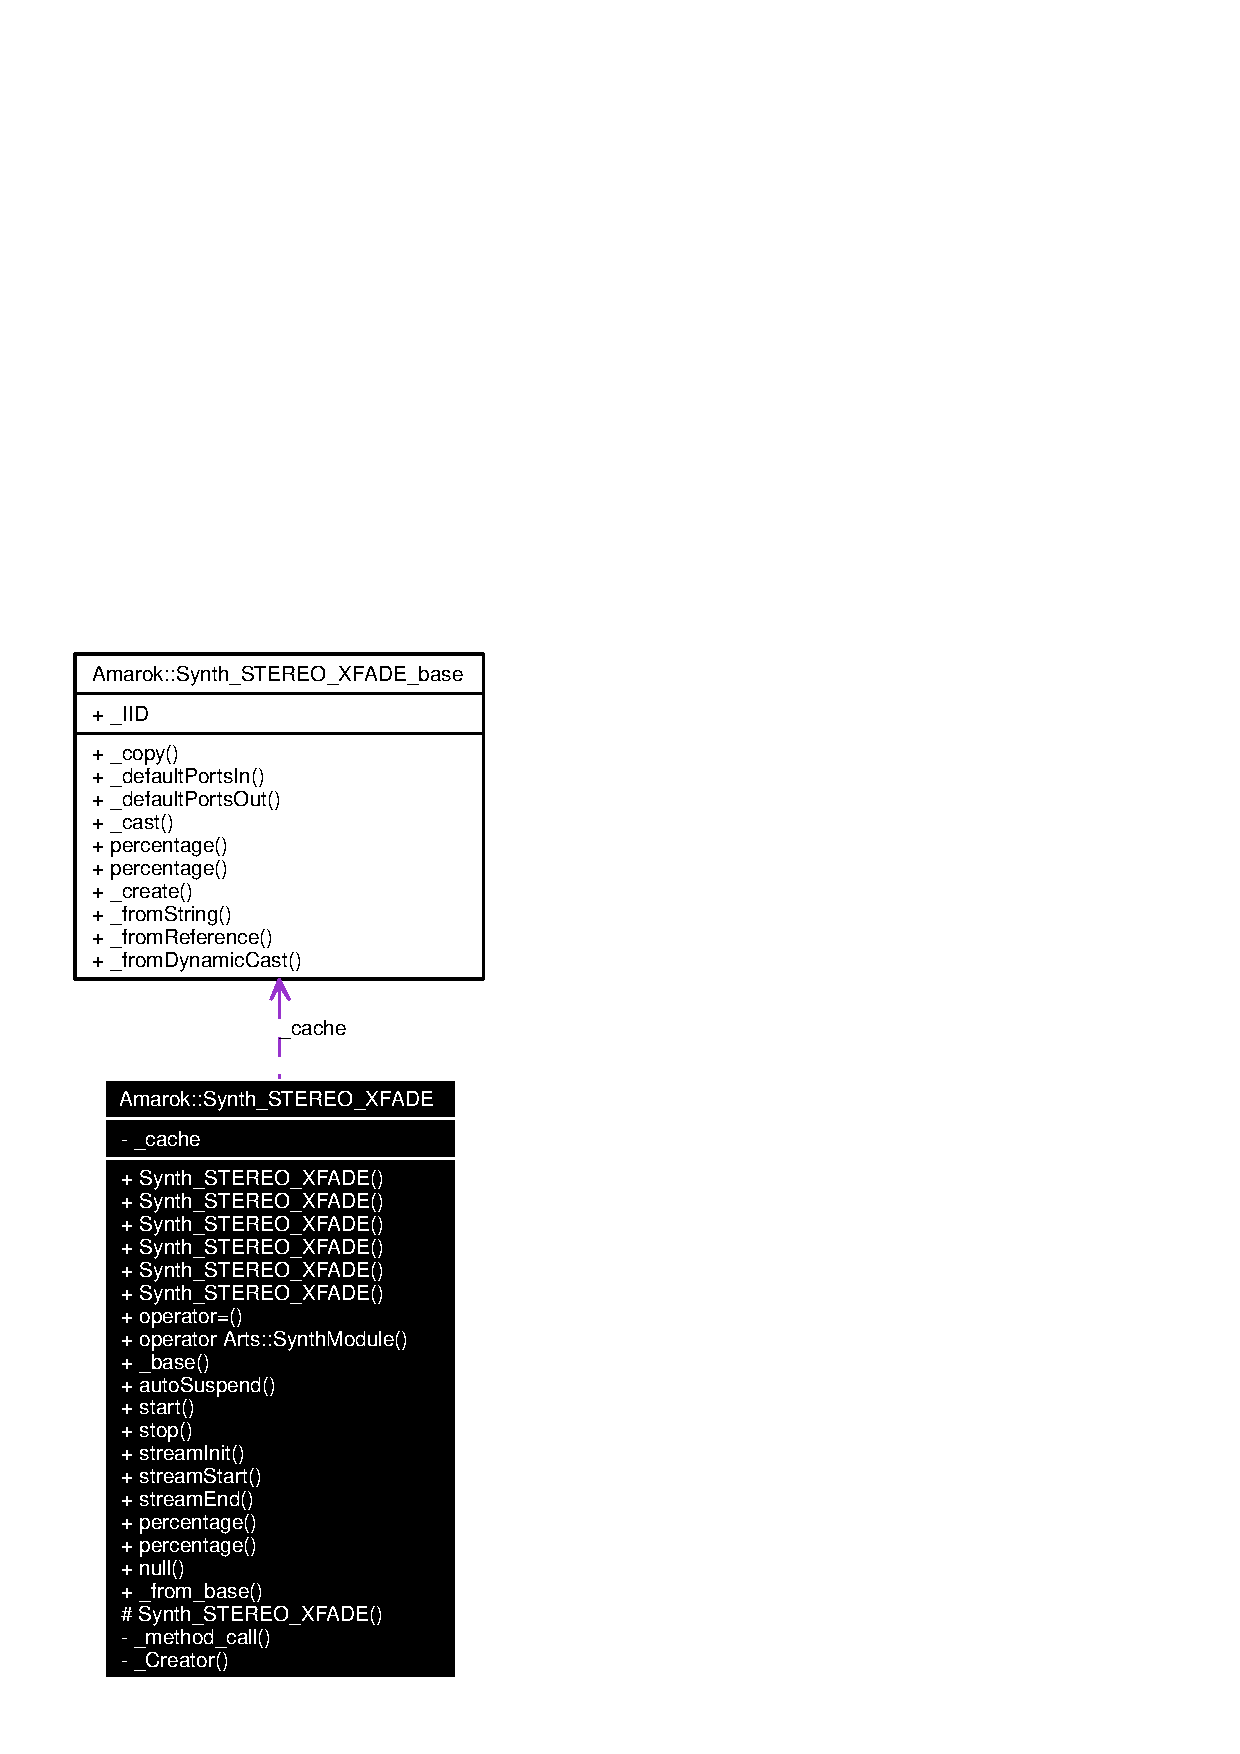
\includegraphics[width=116pt]{classAmarok_1_1Synth__STEREO__XFADE__coll__graph}
\end{center}
\end{figure}
\subsection*{Public Types}
\begin{CompactItemize}
\item 
typedef {\bf Synth\_\-STEREO\_\-XFADE\_\-base} {\bf \_\-base\_\-class}
\end{CompactItemize}
\subsection*{Public Member Functions}
\begin{CompactItemize}
\item 
{\bf Synth\_\-STEREO\_\-XFADE} ()
\item 
{\bf Synth\_\-STEREO\_\-XFADE} (const Arts::Sub\-Class \&s)
\item 
{\bf Synth\_\-STEREO\_\-XFADE} (const Arts::Reference \&r)
\item 
{\bf Synth\_\-STEREO\_\-XFADE} (const Arts::Dynamic\-Cast \&c)
\item 
{\bf Synth\_\-STEREO\_\-XFADE} (const {\bf Synth\_\-STEREO\_\-XFADE} \&target)
\item 
{\bf Synth\_\-STEREO\_\-XFADE} (Arts::Object::Pool \&p)
\item 
{\bf Synth\_\-STEREO\_\-XFADE} \& {\bf operator=} (const {\bf Synth\_\-STEREO\_\-XFADE} \&target)
\item 
{\bf operator Arts::Synth\-Module} () const 
\item 
{\bf Synth\_\-STEREO\_\-XFADE\_\-base} $\ast$ {\bf \_\-base} ()
\item 
Arts::Auto\-Suspend\-State {\bf auto\-Suspend} ()
\item 
void {\bf start} ()
\item 
void {\bf stop} ()
\item 
void {\bf stream\-Init} ()
\item 
void {\bf stream\-Start} ()
\item 
void {\bf stream\-End} ()
\item 
float {\bf percentage} ()
\item 
void {\bf percentage} (float \_\-new\-Value)
\end{CompactItemize}
\subsection*{Static Public Member Functions}
\begin{CompactItemize}
\item 
{\bf Synth\_\-STEREO\_\-XFADE} {\bf null} ()
\item 
{\bf Synth\_\-STEREO\_\-XFADE} {\bf \_\-from\_\-base} ({\bf Synth\_\-STEREO\_\-XFADE\_\-base} $\ast$b)
\end{CompactItemize}
\subsection*{Protected Member Functions}
\begin{CompactItemize}
\item 
{\bf Synth\_\-STEREO\_\-XFADE} ({\bf Synth\_\-STEREO\_\-XFADE\_\-base} $\ast$b)
\end{CompactItemize}
\subsection*{Private Member Functions}
\begin{CompactItemize}
\item 
{\bf Synth\_\-STEREO\_\-XFADE\_\-base} $\ast$ {\bf \_\-method\_\-call} ()
\end{CompactItemize}
\subsection*{Static Private Member Functions}
\begin{CompactItemize}
\item 
Arts::Object\_\-base $\ast$ {\bf \_\-Creator} ()
\end{CompactItemize}
\subsection*{Private Attributes}
\begin{CompactItemize}
\item 
{\bf Synth\_\-STEREO\_\-XFADE\_\-base} $\ast$ {\bf \_\-cache}
\end{CompactItemize}


\subsection{Member Typedef Documentation}
\index{Amarok::Synth_STEREO_XFADE@{Amarok::Synth\_\-STEREO\_\-XFADE}!_base_class@{\_\-base\_\-class}}
\index{_base_class@{\_\-base\_\-class}!Amarok::Synth_STEREO_XFADE@{Amarok::Synth\_\-STEREO\_\-XFADE}}
\subsubsection{\setlength{\rightskip}{0pt plus 5cm}typedef {\bf Synth\_\-STEREO\_\-XFADE\_\-base} {\bf Amarok::Synth\_\-STEREO\_\-XFADE::\_\-base\_\-class}}\label{classAmarok_1_1Synth__STEREO__XFADE_Amarok_1_1Synth__STEREO__XFADEw0}




Definition at line 97 of file amarokarts.h.

\subsection{Constructor \& Destructor Documentation}
\index{Amarok::Synth_STEREO_XFADE@{Amarok::Synth\_\-STEREO\_\-XFADE}!Synth_STEREO_XFADE@{Synth\_\-STEREO\_\-XFADE}}
\index{Synth_STEREO_XFADE@{Synth\_\-STEREO\_\-XFADE}!Amarok::Synth_STEREO_XFADE@{Amarok::Synth\_\-STEREO\_\-XFADE}}
\subsubsection{\setlength{\rightskip}{0pt plus 5cm}Amarok::Synth\_\-STEREO\_\-XFADE::Synth\_\-STEREO\_\-XFADE ({\bf Synth\_\-STEREO\_\-XFADE\_\-base} $\ast$ {\em b})\hspace{0.3cm}{\tt  [inline, protected]}}\label{classAmarok_1_1Synth__STEREO__XFADE_Amarok_1_1Synth__STEREO__XFADEb0}




Definition at line 93 of file amarokarts.h.

References \_\-cache.



\footnotesize\begin{verbatim}93 : Arts::Object(b), _cache(0) {}
\end{verbatim}\normalsize 
\index{Amarok::Synth_STEREO_XFADE@{Amarok::Synth\_\-STEREO\_\-XFADE}!Synth_STEREO_XFADE@{Synth\_\-STEREO\_\-XFADE}}
\index{Synth_STEREO_XFADE@{Synth\_\-STEREO\_\-XFADE}!Amarok::Synth_STEREO_XFADE@{Amarok::Synth\_\-STEREO\_\-XFADE}}
\subsubsection{\setlength{\rightskip}{0pt plus 5cm}Amarok::Synth\_\-STEREO\_\-XFADE::Synth\_\-STEREO\_\-XFADE ()\hspace{0.3cm}{\tt  [inline]}}\label{classAmarok_1_1Synth__STEREO__XFADE_Amarok_1_1Synth__STEREO__XFADEa0}




Definition at line 99 of file amarokarts.h.

References \_\-cache.

Referenced by \_\-from\_\-base(), and null().



\footnotesize\begin{verbatim}99 : Arts::Object(_Creator), _cache(0) {}
\end{verbatim}\normalsize 
\index{Amarok::Synth_STEREO_XFADE@{Amarok::Synth\_\-STEREO\_\-XFADE}!Synth_STEREO_XFADE@{Synth\_\-STEREO\_\-XFADE}}
\index{Synth_STEREO_XFADE@{Synth\_\-STEREO\_\-XFADE}!Amarok::Synth_STEREO_XFADE@{Amarok::Synth\_\-STEREO\_\-XFADE}}
\subsubsection{\setlength{\rightskip}{0pt plus 5cm}Amarok::Synth\_\-STEREO\_\-XFADE::Synth\_\-STEREO\_\-XFADE (const Arts::Sub\-Class \& {\em s})\hspace{0.3cm}{\tt  [inline]}}\label{classAmarok_1_1Synth__STEREO__XFADE_Amarok_1_1Synth__STEREO__XFADEa1}




Definition at line 100 of file amarokarts.h.

References \_\-cache.



\footnotesize\begin{verbatim}100                                                          :
101                 Arts::Object(Synth_STEREO_XFADE_base::_create(s.string())), _cache(0) {}
        inline Synth_STEREO_XFADE(const Arts::Reference &r) :
\end{verbatim}\normalsize 
\index{Amarok::Synth_STEREO_XFADE@{Amarok::Synth\_\-STEREO\_\-XFADE}!Synth_STEREO_XFADE@{Synth\_\-STEREO\_\-XFADE}}
\index{Synth_STEREO_XFADE@{Synth\_\-STEREO\_\-XFADE}!Amarok::Synth_STEREO_XFADE@{Amarok::Synth\_\-STEREO\_\-XFADE}}
\subsubsection{\setlength{\rightskip}{0pt plus 5cm}Amarok::Synth\_\-STEREO\_\-XFADE::Synth\_\-STEREO\_\-XFADE (const Arts::Reference \& {\em r})\hspace{0.3cm}{\tt  [inline]}}\label{classAmarok_1_1Synth__STEREO__XFADE_Amarok_1_1Synth__STEREO__XFADEa2}




Definition at line 102 of file amarokarts.h.

References \_\-cache.



\footnotesize\begin{verbatim}102                                                           :
103                 Arts::Object(r.isString()?(Synth_STEREO_XFADE_base::_fromString(r.string())):(Synth_STEREO_XFADE_base::_fromReference(r.reference(),true))), _cache(0) {}
        inline Synth_STEREO_XFADE(const Arts::DynamicCast& c) : Arts::Object(Synth_STEREO_XFADE_base::_fromDynamicCast(c.object())), _cache(0) {}
\end{verbatim}\normalsize 
\index{Amarok::Synth_STEREO_XFADE@{Amarok::Synth\_\-STEREO\_\-XFADE}!Synth_STEREO_XFADE@{Synth\_\-STEREO\_\-XFADE}}
\index{Synth_STEREO_XFADE@{Synth\_\-STEREO\_\-XFADE}!Amarok::Synth_STEREO_XFADE@{Amarok::Synth\_\-STEREO\_\-XFADE}}
\subsubsection{\setlength{\rightskip}{0pt plus 5cm}Amarok::Synth\_\-STEREO\_\-XFADE::Synth\_\-STEREO\_\-XFADE (const Arts::Dynamic\-Cast \& {\em c})\hspace{0.3cm}{\tt  [inline]}}\label{classAmarok_1_1Synth__STEREO__XFADE_Amarok_1_1Synth__STEREO__XFADEa3}




Definition at line 104 of file amarokarts.h.

References \_\-cache.



\footnotesize\begin{verbatim}104 : Arts::Object(Synth_STEREO_XFADE_base::_fromDynamicCast(c.object())), _cache(0) {}
\end{verbatim}\normalsize 
\index{Amarok::Synth_STEREO_XFADE@{Amarok::Synth\_\-STEREO\_\-XFADE}!Synth_STEREO_XFADE@{Synth\_\-STEREO\_\-XFADE}}
\index{Synth_STEREO_XFADE@{Synth\_\-STEREO\_\-XFADE}!Amarok::Synth_STEREO_XFADE@{Amarok::Synth\_\-STEREO\_\-XFADE}}
\subsubsection{\setlength{\rightskip}{0pt plus 5cm}Amarok::Synth\_\-STEREO\_\-XFADE::Synth\_\-STEREO\_\-XFADE (const {\bf Synth\_\-STEREO\_\-XFADE} \& {\em target})\hspace{0.3cm}{\tt  [inline]}}\label{classAmarok_1_1Synth__STEREO__XFADE_Amarok_1_1Synth__STEREO__XFADEa4}




Definition at line 105 of file amarokarts.h.

References \_\-cache.



\footnotesize\begin{verbatim}105 : Arts::Object(target._pool), _cache(target._cache) {}
\end{verbatim}\normalsize 
\index{Amarok::Synth_STEREO_XFADE@{Amarok::Synth\_\-STEREO\_\-XFADE}!Synth_STEREO_XFADE@{Synth\_\-STEREO\_\-XFADE}}
\index{Synth_STEREO_XFADE@{Synth\_\-STEREO\_\-XFADE}!Amarok::Synth_STEREO_XFADE@{Amarok::Synth\_\-STEREO\_\-XFADE}}
\subsubsection{\setlength{\rightskip}{0pt plus 5cm}Amarok::Synth\_\-STEREO\_\-XFADE::Synth\_\-STEREO\_\-XFADE (Arts::Object::Pool \& {\em p})\hspace{0.3cm}{\tt  [inline]}}\label{classAmarok_1_1Synth__STEREO__XFADE_Amarok_1_1Synth__STEREO__XFADEa5}




Definition at line 106 of file amarokarts.h.

References \_\-cache.



\footnotesize\begin{verbatim}106 : Arts::Object(p), _cache(0) {}
\end{verbatim}\normalsize 


\subsection{Member Function Documentation}
\index{Amarok::Synth_STEREO_XFADE@{Amarok::Synth\_\-STEREO\_\-XFADE}!_base@{\_\-base}}
\index{_base@{\_\-base}!Amarok::Synth_STEREO_XFADE@{Amarok::Synth\_\-STEREO\_\-XFADE}}
\subsubsection{\setlength{\rightskip}{0pt plus 5cm}{\bf Synth\_\-STEREO\_\-XFADE\_\-base}$\ast$ Amarok::Synth\_\-STEREO\_\-XFADE::\_\-base ()\hspace{0.3cm}{\tt  [inline]}}\label{classAmarok_1_1Synth__STEREO__XFADE_Amarok_1_1Synth__STEREO__XFADEa8}




Definition at line 118 of file amarokarts.h.



\footnotesize\begin{verbatim}118 {return _cache?_cache:_method_call();}
\end{verbatim}\normalsize 
\index{Amarok::Synth_STEREO_XFADE@{Amarok::Synth\_\-STEREO\_\-XFADE}!_Creator@{\_\-Creator}}
\index{_Creator@{\_\-Creator}!Amarok::Synth_STEREO_XFADE@{Amarok::Synth\_\-STEREO\_\-XFADE}}
\subsubsection{\setlength{\rightskip}{0pt plus 5cm}Arts::Object\_\-base $\ast$ Amarok::Synth\_\-STEREO\_\-XFADE::\_\-Creator ()\hspace{0.3cm}{\tt  [static, private]}}\label{classAmarok_1_1Synth__STEREO__XFADE_Amarok_1_1Synth__STEREO__XFADEh0}




Definition at line 176 of file amarokarts.cc.

References Amarok::Synth\_\-STEREO\_\-XFADE\_\-base::\_\-create().



\footnotesize\begin{verbatim}176                                                     {
177         return Amarok::Synth_STEREO_XFADE_base::_create();
178 }
\end{verbatim}\normalsize 


Here is the call graph for this function:\begin{figure}[H]
\begin{center}
\leavevmode
\includegraphics[width=261pt]{classAmarok_1_1Synth__STEREO__XFADE_Amarok_1_1Synth__STEREO__XFADEh0_cgraph}
\end{center}
\end{figure}
\index{Amarok::Synth_STEREO_XFADE@{Amarok::Synth\_\-STEREO\_\-XFADE}!_from_base@{\_\-from\_\-base}}
\index{_from_base@{\_\-from\_\-base}!Amarok::Synth_STEREO_XFADE@{Amarok::Synth\_\-STEREO\_\-XFADE}}
\subsubsection{\setlength{\rightskip}{0pt plus 5cm}{\bf Synth\_\-STEREO\_\-XFADE} Amarok::Synth\_\-STEREO\_\-XFADE::\_\-from\_\-base ({\bf Synth\_\-STEREO\_\-XFADE\_\-base} $\ast$ {\em b})\hspace{0.3cm}{\tt  [inline, static]}}\label{classAmarok_1_1Synth__STEREO__XFADE_Amarok_1_1Synth__STEREO__XFADEe1}




Definition at line 108 of file amarokarts.h.

References Synth\_\-STEREO\_\-XFADE().



\footnotesize\begin{verbatim}108 {return Synth_STEREO_XFADE(b);}
\end{verbatim}\normalsize 


Here is the call graph for this function:\begin{figure}[H]
\begin{center}
\leavevmode
\includegraphics[width=293pt]{classAmarok_1_1Synth__STEREO__XFADE_Amarok_1_1Synth__STEREO__XFADEe1_cgraph}
\end{center}
\end{figure}
\index{Amarok::Synth_STEREO_XFADE@{Amarok::Synth\_\-STEREO\_\-XFADE}!_method_call@{\_\-method\_\-call}}
\index{_method_call@{\_\-method\_\-call}!Amarok::Synth_STEREO_XFADE@{Amarok::Synth\_\-STEREO\_\-XFADE}}
\subsubsection{\setlength{\rightskip}{0pt plus 5cm}{\bf Synth\_\-STEREO\_\-XFADE\_\-base}$\ast$ Amarok::Synth\_\-STEREO\_\-XFADE::\_\-method\_\-call ()\hspace{0.3cm}{\tt  [inline, private]}}\label{classAmarok_1_1Synth__STEREO__XFADE_Amarok_1_1Synth__STEREO__XFADEd0}




Definition at line 83 of file amarokarts.h.

References \_\-cache, and Amarok::Synth\_\-STEREO\_\-XFADE\_\-base::\_\-cast().

Referenced by auto\-Suspend(), percentage(), start(), stop(), stream\-End(), stream\-Init(), and stream\-Start().



\footnotesize\begin{verbatim}83                                                        {
84                 _pool->checkcreate();
85                 if(_pool->base) {
86                         _cache=(Synth_STEREO_XFADE_base *)_pool->base->_cast(Synth_STEREO_XFADE_base::_IID);
87                         assert(_cache);
88                 }
89                 return _cache;
90         }
\end{verbatim}\normalsize 


Here is the call graph for this function:\begin{figure}[H]
\begin{center}
\leavevmode
\includegraphics[width=266pt]{classAmarok_1_1Synth__STEREO__XFADE_Amarok_1_1Synth__STEREO__XFADEd0_cgraph}
\end{center}
\end{figure}
\index{Amarok::Synth_STEREO_XFADE@{Amarok::Synth\_\-STEREO\_\-XFADE}!autoSuspend@{autoSuspend}}
\index{autoSuspend@{autoSuspend}!Amarok::Synth_STEREO_XFADE@{Amarok::Synth\_\-STEREO\_\-XFADE}}
\subsubsection{\setlength{\rightskip}{0pt plus 5cm}Arts::Auto\-Suspend\-State Amarok::Synth\_\-STEREO\_\-XFADE::auto\-Suspend ()\hspace{0.3cm}{\tt  [inline]}}\label{classAmarok_1_1Synth__STEREO__XFADE_Amarok_1_1Synth__STEREO__XFADEa9}




Definition at line 243 of file amarokarts.h.

References \_\-cache, and \_\-method\_\-call().



\footnotesize\begin{verbatim}244 {
245         return _cache?static_cast<Arts::SynthModule_base*>(_cache)->autoSuspend():static_cast<Arts::SynthModule_base*>(_method_call())->autoSuspend();
246 }
\end{verbatim}\normalsize 


Here is the call graph for this function:\begin{figure}[H]
\begin{center}
\leavevmode
\includegraphics[width=401pt]{classAmarok_1_1Synth__STEREO__XFADE_Amarok_1_1Synth__STEREO__XFADEa9_cgraph}
\end{center}
\end{figure}
\index{Amarok::Synth_STEREO_XFADE@{Amarok::Synth\_\-STEREO\_\-XFADE}!null@{null}}
\index{null@{null}!Amarok::Synth_STEREO_XFADE@{Amarok::Synth\_\-STEREO\_\-XFADE}}
\subsubsection{\setlength{\rightskip}{0pt plus 5cm}{\bf Synth\_\-STEREO\_\-XFADE} Amarok::Synth\_\-STEREO\_\-XFADE::null ()\hspace{0.3cm}{\tt  [inline, static]}}\label{classAmarok_1_1Synth__STEREO__XFADE_Amarok_1_1Synth__STEREO__XFADEe0}




Definition at line 107 of file amarokarts.h.

References Synth\_\-STEREO\_\-XFADE().

Referenced by Arts\-Engine::$\sim$Arts\-Engine().



\footnotesize\begin{verbatim}107 {return Synth_STEREO_XFADE((Synth_STEREO_XFADE_base*)0);}
\end{verbatim}\normalsize 


Here is the call graph for this function:\begin{figure}[H]
\begin{center}
\leavevmode
\includegraphics[width=274pt]{classAmarok_1_1Synth__STEREO__XFADE_Amarok_1_1Synth__STEREO__XFADEe0_cgraph}
\end{center}
\end{figure}
\index{Amarok::Synth_STEREO_XFADE@{Amarok::Synth\_\-STEREO\_\-XFADE}!operator Arts::SynthModule@{operator Arts::SynthModule}}
\index{operator Arts::SynthModule@{operator Arts::SynthModule}!Amarok::Synth_STEREO_XFADE@{Amarok::Synth\_\-STEREO\_\-XFADE}}
\subsubsection{\setlength{\rightskip}{0pt plus 5cm}Amarok::Synth\_\-STEREO\_\-XFADE::operator Arts::Synth\-Module () const\hspace{0.3cm}{\tt  [inline]}}\label{classAmarok_1_1Synth__STEREO__XFADE_Amarok_1_1Synth__STEREO__XFADEa7}




Definition at line 117 of file amarokarts.h.

References operator Arts::Synth\-Module().

Referenced by operator Arts::Synth\-Module().



\footnotesize\begin{verbatim}117 { return Arts::SynthModule(*_pool); }
\end{verbatim}\normalsize 


Here is the call graph for this function:\begin{figure}[H]
\begin{center}
\leavevmode
\includegraphics[width=135pt]{classAmarok_1_1Synth__STEREO__XFADE_Amarok_1_1Synth__STEREO__XFADEa7_cgraph}
\end{center}
\end{figure}
\index{Amarok::Synth_STEREO_XFADE@{Amarok::Synth\_\-STEREO\_\-XFADE}!operator=@{operator=}}
\index{operator=@{operator=}!Amarok::Synth_STEREO_XFADE@{Amarok::Synth\_\-STEREO\_\-XFADE}}
\subsubsection{\setlength{\rightskip}{0pt plus 5cm}{\bf Synth\_\-STEREO\_\-XFADE}\& Amarok::Synth\_\-STEREO\_\-XFADE::operator= (const {\bf Synth\_\-STEREO\_\-XFADE} \& {\em target})\hspace{0.3cm}{\tt  [inline]}}\label{classAmarok_1_1Synth__STEREO__XFADE_Amarok_1_1Synth__STEREO__XFADEa6}




Definition at line 109 of file amarokarts.h.

References \_\-cache.



\footnotesize\begin{verbatim}109                                                                                {
110                 if (_pool == target._pool) return *this;
111                 _pool->Dec();
112                 _pool = target._pool;
113                 _cache = target._cache;
114                 _pool->Inc();
115                 return *this;
116         }
\end{verbatim}\normalsize 
\index{Amarok::Synth_STEREO_XFADE@{Amarok::Synth\_\-STEREO\_\-XFADE}!percentage@{percentage}}
\index{percentage@{percentage}!Amarok::Synth_STEREO_XFADE@{Amarok::Synth\_\-STEREO\_\-XFADE}}
\subsubsection{\setlength{\rightskip}{0pt plus 5cm}void Amarok::Synth\_\-STEREO\_\-XFADE::percentage (float {\em \_\-new\-Value})\hspace{0.3cm}{\tt  [inline]}}\label{classAmarok_1_1Synth__STEREO__XFADE_Amarok_1_1Synth__STEREO__XFADEa16}




Definition at line 278 of file amarokarts.h.

References \_\-cache, \_\-method\_\-call(), and Amarok::Synth\_\-STEREO\_\-XFADE\_\-base::percentage().



\footnotesize\begin{verbatim}279 {
280          _cache?static_cast<Amarok::Synth_STEREO_XFADE_base*>(_cache)->percentage(_newValue):static_cast<Amarok::Synth_STEREO_XFADE_base*>(_method_call())->percentage(_newValue);
281 }
\end{verbatim}\normalsize 


Here is the call graph for this function:\begin{figure}[H]
\begin{center}
\leavevmode
\includegraphics[width=275pt]{classAmarok_1_1Synth__STEREO__XFADE_Amarok_1_1Synth__STEREO__XFADEa16_cgraph}
\end{center}
\end{figure}
\index{Amarok::Synth_STEREO_XFADE@{Amarok::Synth\_\-STEREO\_\-XFADE}!percentage@{percentage}}
\index{percentage@{percentage}!Amarok::Synth_STEREO_XFADE@{Amarok::Synth\_\-STEREO\_\-XFADE}}
\subsubsection{\setlength{\rightskip}{0pt plus 5cm}float Amarok::Synth\_\-STEREO\_\-XFADE::percentage ()\hspace{0.3cm}{\tt  [inline]}}\label{classAmarok_1_1Synth__STEREO__XFADE_Amarok_1_1Synth__STEREO__XFADEa15}




Definition at line 273 of file amarokarts.h.

References \_\-cache, \_\-method\_\-call(), and Amarok::Synth\_\-STEREO\_\-XFADE\_\-base::percentage().

Referenced by Arts\-Engine::init(), and Arts\-Engine::timer\-Event().



\footnotesize\begin{verbatim}274 {
275         return _cache?static_cast<Amarok::Synth_STEREO_XFADE_base*>(_cache)->percentage():static_cast<Amarok::Synth_STEREO_XFADE_base*>(_method_call())->percentage();
276 }
\end{verbatim}\normalsize 


Here is the call graph for this function:\begin{figure}[H]
\begin{center}
\leavevmode
\includegraphics[width=275pt]{classAmarok_1_1Synth__STEREO__XFADE_Amarok_1_1Synth__STEREO__XFADEa15_cgraph}
\end{center}
\end{figure}
\index{Amarok::Synth_STEREO_XFADE@{Amarok::Synth\_\-STEREO\_\-XFADE}!start@{start}}
\index{start@{start}!Amarok::Synth_STEREO_XFADE@{Amarok::Synth\_\-STEREO\_\-XFADE}}
\subsubsection{\setlength{\rightskip}{0pt plus 5cm}void Amarok::Synth\_\-STEREO\_\-XFADE::start ()\hspace{0.3cm}{\tt  [inline]}}\label{classAmarok_1_1Synth__STEREO__XFADE_Amarok_1_1Synth__STEREO__XFADEa10}




Definition at line 248 of file amarokarts.h.

References \_\-cache, and \_\-method\_\-call().

Referenced by Arts\-Engine::init().



\footnotesize\begin{verbatim}249 {
250          _cache?static_cast<Arts::SynthModule_base*>(_cache)->start():static_cast<Arts::SynthModule_base*>(_method_call())->start();
251 }
\end{verbatim}\normalsize 


Here is the call graph for this function:\begin{figure}[H]
\begin{center}
\leavevmode
\includegraphics[width=382pt]{classAmarok_1_1Synth__STEREO__XFADE_Amarok_1_1Synth__STEREO__XFADEa10_cgraph}
\end{center}
\end{figure}
\index{Amarok::Synth_STEREO_XFADE@{Amarok::Synth\_\-STEREO\_\-XFADE}!stop@{stop}}
\index{stop@{stop}!Amarok::Synth_STEREO_XFADE@{Amarok::Synth\_\-STEREO\_\-XFADE}}
\subsubsection{\setlength{\rightskip}{0pt plus 5cm}void Amarok::Synth\_\-STEREO\_\-XFADE::stop ()\hspace{0.3cm}{\tt  [inline]}}\label{classAmarok_1_1Synth__STEREO__XFADE_Amarok_1_1Synth__STEREO__XFADEa11}




Definition at line 253 of file amarokarts.h.

References \_\-cache, and \_\-method\_\-call().



\footnotesize\begin{verbatim}254 {
255          _cache?static_cast<Arts::SynthModule_base*>(_cache)->stop():static_cast<Arts::SynthModule_base*>(_method_call())->stop();
256 }
\end{verbatim}\normalsize 


Here is the call graph for this function:\begin{figure}[H]
\begin{center}
\leavevmode
\includegraphics[width=381pt]{classAmarok_1_1Synth__STEREO__XFADE_Amarok_1_1Synth__STEREO__XFADEa11_cgraph}
\end{center}
\end{figure}
\index{Amarok::Synth_STEREO_XFADE@{Amarok::Synth\_\-STEREO\_\-XFADE}!streamEnd@{streamEnd}}
\index{streamEnd@{streamEnd}!Amarok::Synth_STEREO_XFADE@{Amarok::Synth\_\-STEREO\_\-XFADE}}
\subsubsection{\setlength{\rightskip}{0pt plus 5cm}void Amarok::Synth\_\-STEREO\_\-XFADE::stream\-End ()\hspace{0.3cm}{\tt  [inline]}}\label{classAmarok_1_1Synth__STEREO__XFADE_Amarok_1_1Synth__STEREO__XFADEa14}




Definition at line 268 of file amarokarts.h.

References \_\-cache, and \_\-method\_\-call().



\footnotesize\begin{verbatim}269 {
270          _cache?static_cast<Arts::SynthModule_base*>(_cache)->streamEnd():static_cast<Arts::SynthModule_base*>(_method_call())->streamEnd();
271 }
\end{verbatim}\normalsize 


Here is the call graph for this function:\begin{figure}[H]
\begin{center}
\leavevmode
\includegraphics[width=396pt]{classAmarok_1_1Synth__STEREO__XFADE_Amarok_1_1Synth__STEREO__XFADEa14_cgraph}
\end{center}
\end{figure}
\index{Amarok::Synth_STEREO_XFADE@{Amarok::Synth\_\-STEREO\_\-XFADE}!streamInit@{streamInit}}
\index{streamInit@{streamInit}!Amarok::Synth_STEREO_XFADE@{Amarok::Synth\_\-STEREO\_\-XFADE}}
\subsubsection{\setlength{\rightskip}{0pt plus 5cm}void Amarok::Synth\_\-STEREO\_\-XFADE::stream\-Init ()\hspace{0.3cm}{\tt  [inline]}}\label{classAmarok_1_1Synth__STEREO__XFADE_Amarok_1_1Synth__STEREO__XFADEa12}




Definition at line 258 of file amarokarts.h.

References \_\-cache, and \_\-method\_\-call().



\footnotesize\begin{verbatim}259 {
260          _cache?static_cast<Arts::SynthModule_base*>(_cache)->streamInit():static_cast<Arts::SynthModule_base*>(_method_call())->streamInit();
261 }
\end{verbatim}\normalsize 


Here is the call graph for this function:\begin{figure}[H]
\begin{center}
\leavevmode
\includegraphics[width=394pt]{classAmarok_1_1Synth__STEREO__XFADE_Amarok_1_1Synth__STEREO__XFADEa12_cgraph}
\end{center}
\end{figure}
\index{Amarok::Synth_STEREO_XFADE@{Amarok::Synth\_\-STEREO\_\-XFADE}!streamStart@{streamStart}}
\index{streamStart@{streamStart}!Amarok::Synth_STEREO_XFADE@{Amarok::Synth\_\-STEREO\_\-XFADE}}
\subsubsection{\setlength{\rightskip}{0pt plus 5cm}void Amarok::Synth\_\-STEREO\_\-XFADE::stream\-Start ()\hspace{0.3cm}{\tt  [inline]}}\label{classAmarok_1_1Synth__STEREO__XFADE_Amarok_1_1Synth__STEREO__XFADEa13}




Definition at line 263 of file amarokarts.h.

References \_\-cache, and \_\-method\_\-call().



\footnotesize\begin{verbatim}264 {
265          _cache?static_cast<Arts::SynthModule_base*>(_cache)->streamStart():static_cast<Arts::SynthModule_base*>(_method_call())->streamStart();
266 }
\end{verbatim}\normalsize 


Here is the call graph for this function:\begin{figure}[H]
\begin{center}
\leavevmode
\includegraphics[width=398pt]{classAmarok_1_1Synth__STEREO__XFADE_Amarok_1_1Synth__STEREO__XFADEa13_cgraph}
\end{center}
\end{figure}


\subsection{Member Data Documentation}
\index{Amarok::Synth_STEREO_XFADE@{Amarok::Synth\_\-STEREO\_\-XFADE}!_cache@{\_\-cache}}
\index{_cache@{\_\-cache}!Amarok::Synth_STEREO_XFADE@{Amarok::Synth\_\-STEREO\_\-XFADE}}
\subsubsection{\setlength{\rightskip}{0pt plus 5cm}{\bf Synth\_\-STEREO\_\-XFADE\_\-base}$\ast$ {\bf Amarok::Synth\_\-STEREO\_\-XFADE::\_\-cache}\hspace{0.3cm}{\tt  [private]}}\label{classAmarok_1_1Synth__STEREO__XFADE_Amarok_1_1Synth__STEREO__XFADEr0}




Definition at line 82 of file amarokarts.h.

Referenced by \_\-method\_\-call(), auto\-Suspend(), operator=(), percentage(), start(), stop(), stream\-End(), stream\-Init(), stream\-Start(), and Synth\_\-STEREO\_\-XFADE().

The documentation for this class was generated from the following files:\begin{CompactItemize}
\item 
{\bf amarokarts.h}\item 
{\bf amarokarts.cc}\end{CompactItemize}
